\chapter{MSX System Architecture}

\section{Overview of an MSX computer}

We can start this book providing a bird’s sight of how an MSX computer is made. It might be obvious, but you will have to understand how an MSX computer works at its highest level before understanding how an Artemisa computer is designed.\\

Most 8-bit microcomputers are amazingly simple. They include a CPU, a few tens of kilobytes of memory and some peripherals. All of them connected through a \toref{system bus}, as shown in Figure \ref{fig:msx-arch-overview}

\begin{figure}
	\centering
	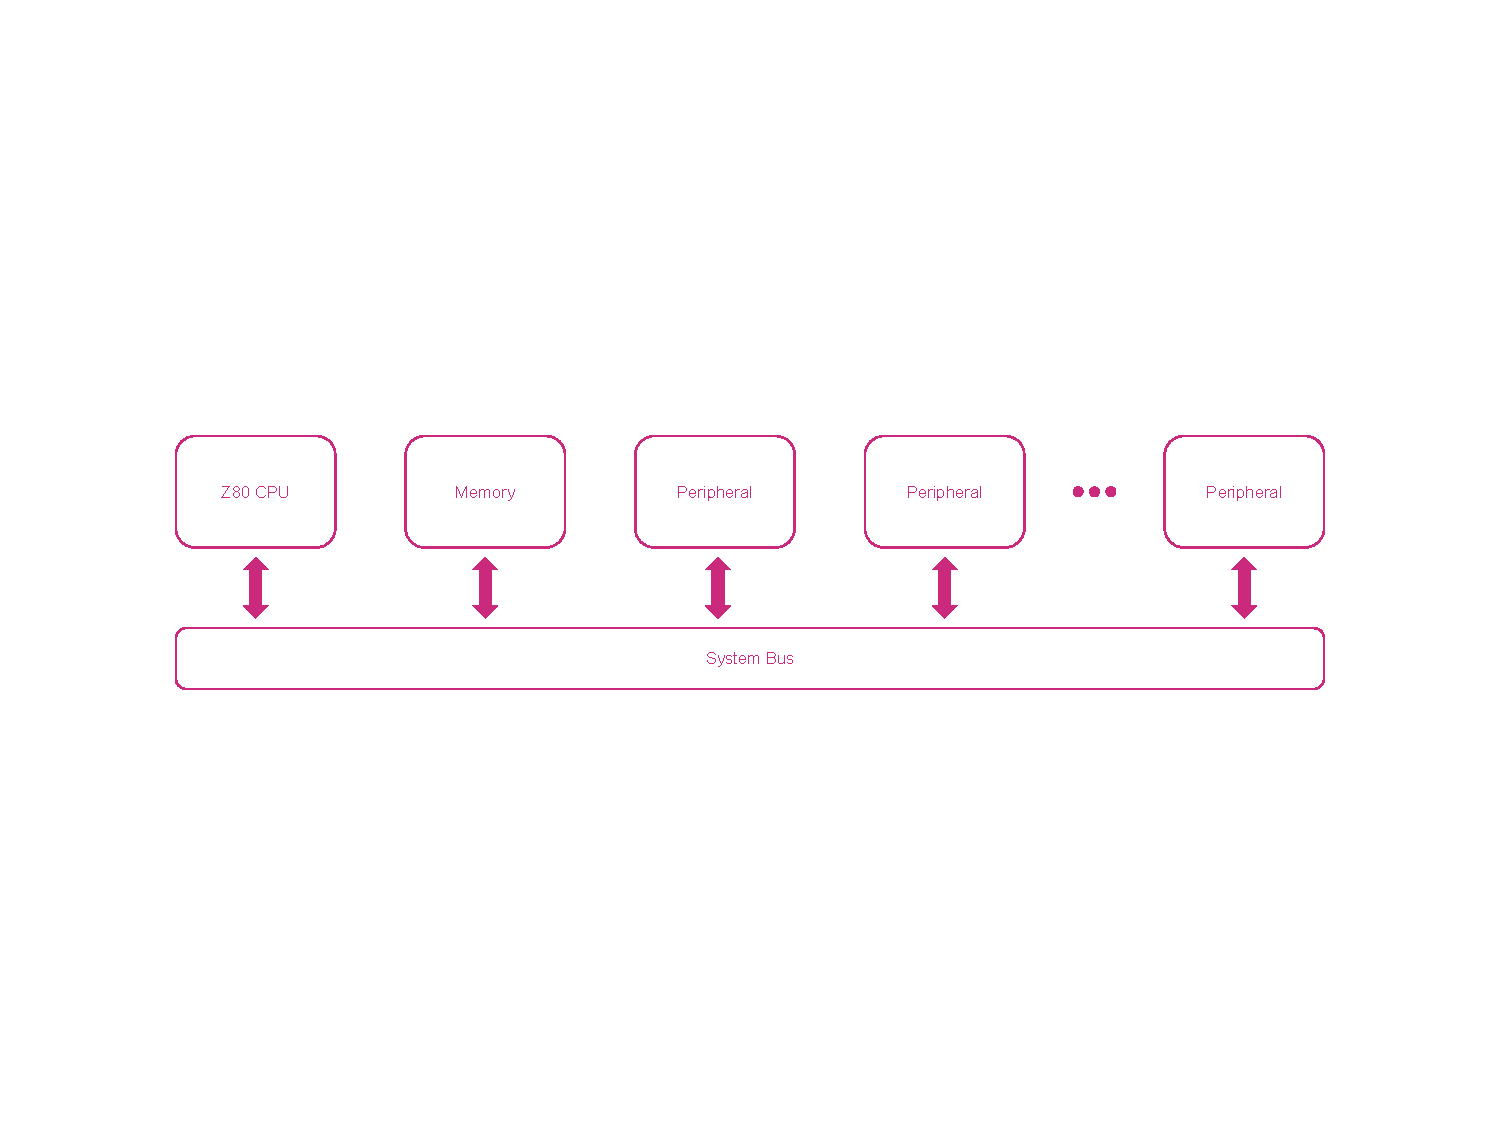
\includegraphics[width=\linewidth,trim={0cm 200 0 200}]{images/figures/msx-arch-overview}
	\caption{High level architecture of a MSX computer}
	\label{fig:msx-arch-overview}
\end{figure}

\begin{theory}{Electronic buses}
	The basic operation of any computer is to move information around. The information is physically represented by electrical wires that may have or not voltage and current. We could simplify this idea by saying that the presence of electrical current and voltage represents the digital number 1, while the absence of it represents the 0. Hence, every single wire can transfer one bit of information at any time.\\\\
	
	A bus in electronics is just a group of wires that have some common purpose. There are some buses that tie the wires together to represent multi-bit magnitudes. For example, if we put 8 wires together, we will have the ability to represent 8-bit numbers. This is a value from 0 to 255 (or -127 to 128). With 16 wires we will represent values from 0 to 65535 (or -32768 to 32767). And so on. Some other times we put wires in the same bus because they represent some information that is closely related. For example, some control signals can be grouped together in the same bus to communicate control actions from one device to another, such as read, write, reset, interrupt, etc. \\\\
	
	If we make an analogy between a computer and the human body, the system bus is the nervous system. In our bodies, it is the medium to transfer the signals from the brain to the muscles to coordinate our actions. But it is also the channel to carry the sensitive information from our five senses to perceive the world. In our computers, the CPU is the brain and the muscles and senses are the peripherals. And all them use the system bus as a kind of nervous system to transfer information in both directions.	
\end{theory}

\subsection{The microprocessor}

The CPU of an MSX computer is a Zilog Z80 microprocessor running at 3.58Mhz. The Z80 was introduced by Zilog in 1976 as an enhancement and direct competitor of the popular Intel 8080. It was binary compatible with the Intel CPU, which means it can execute programs originally created for the 8080. Thanks to this and its extended instruction set, it was positioned as one of the most successful CPUs of all the times. It was chosen by Sinclair to make most of their computers, including the top selling ZX Spectrum. It was also the CPU behind the Amstrad CPC series, and some other game consoles such as the ColecoVision and the Sega Master System. And, of course, it is the brain of any MSX computer system. 

\subsection{The memory}

The memory system of an MSX system is comprised by RAM (typically 64KB) and ROM (typically 32KB) memory. The ROM memory is a read-only memory whose content is written during the manufacturing process. It is used to store the \toref{MSX BIOS} and the MSX Basic interpreter. The RAM memory, in contrast, can be read and write. It is used to store the programs that are loaded from storage devices such as the cassette tape or the floppy drive, and to store the data used by these programs. The RAM memory is volatile, which means its contents will be lost after power off or reset. In contrast, the ROM memory is persistent. Once written during the manufacturing process, its contents will persist until the end of the days or until it is destroyed. The thing that happens first.\\

However, the memory system of the MSX is quite complex. It has a sophisticated bank switching mechanism to break the limit of 64KB of memory space of the Z80 CPU, as we will see later in detail in page \pageref{sec:msx-mem-slots}. Hence, it uses a not trivial decoding and slot selection logic to interpret the signals coming from the system bus and the Parallel Peripheral Interface (PPI) in order to identify the memory device when it is addressed, as shown in Figure \ref{fig:msx-arch-memory}. Do not worry about PPI for now, we will cover this later. \\

\begin{theory}{The MSX BIOS}
	BIOS is the acronym of Basic Input/Output System. This is an essential software program present in any computer system that serves two purposes.\\\\
	
	First, it is the first software the CPU will execute upon boot. Thus, it is responsible of preparing the system before the first program can run. Here preparing the system means initializing the hardware into a consistent state, perform a few sanity-checks to ensure the hardware is not malfunctioning and locate the first program that will run. This first program is typically an operating system. In our case, the MSX Basic or the MSX DOS.\\\\
	
	The second purpose is to provide a software abstraction layer over the hardware. The BIOS is a sort of software library that provides utility routines the programmer can use to interact with the hardware. This not only simplifies the life of the programmers, but also ensures the portability of their programs. The BIOS hides the divergencies of the hardware behind an API (Application Programming Interface). So in case of a computer having a different hardware, it is possible to reprogram its BIOS to deal with the differences so that the user software can also run on it without any change. 	
\end{theory}

\begin{figure}
	\centering
	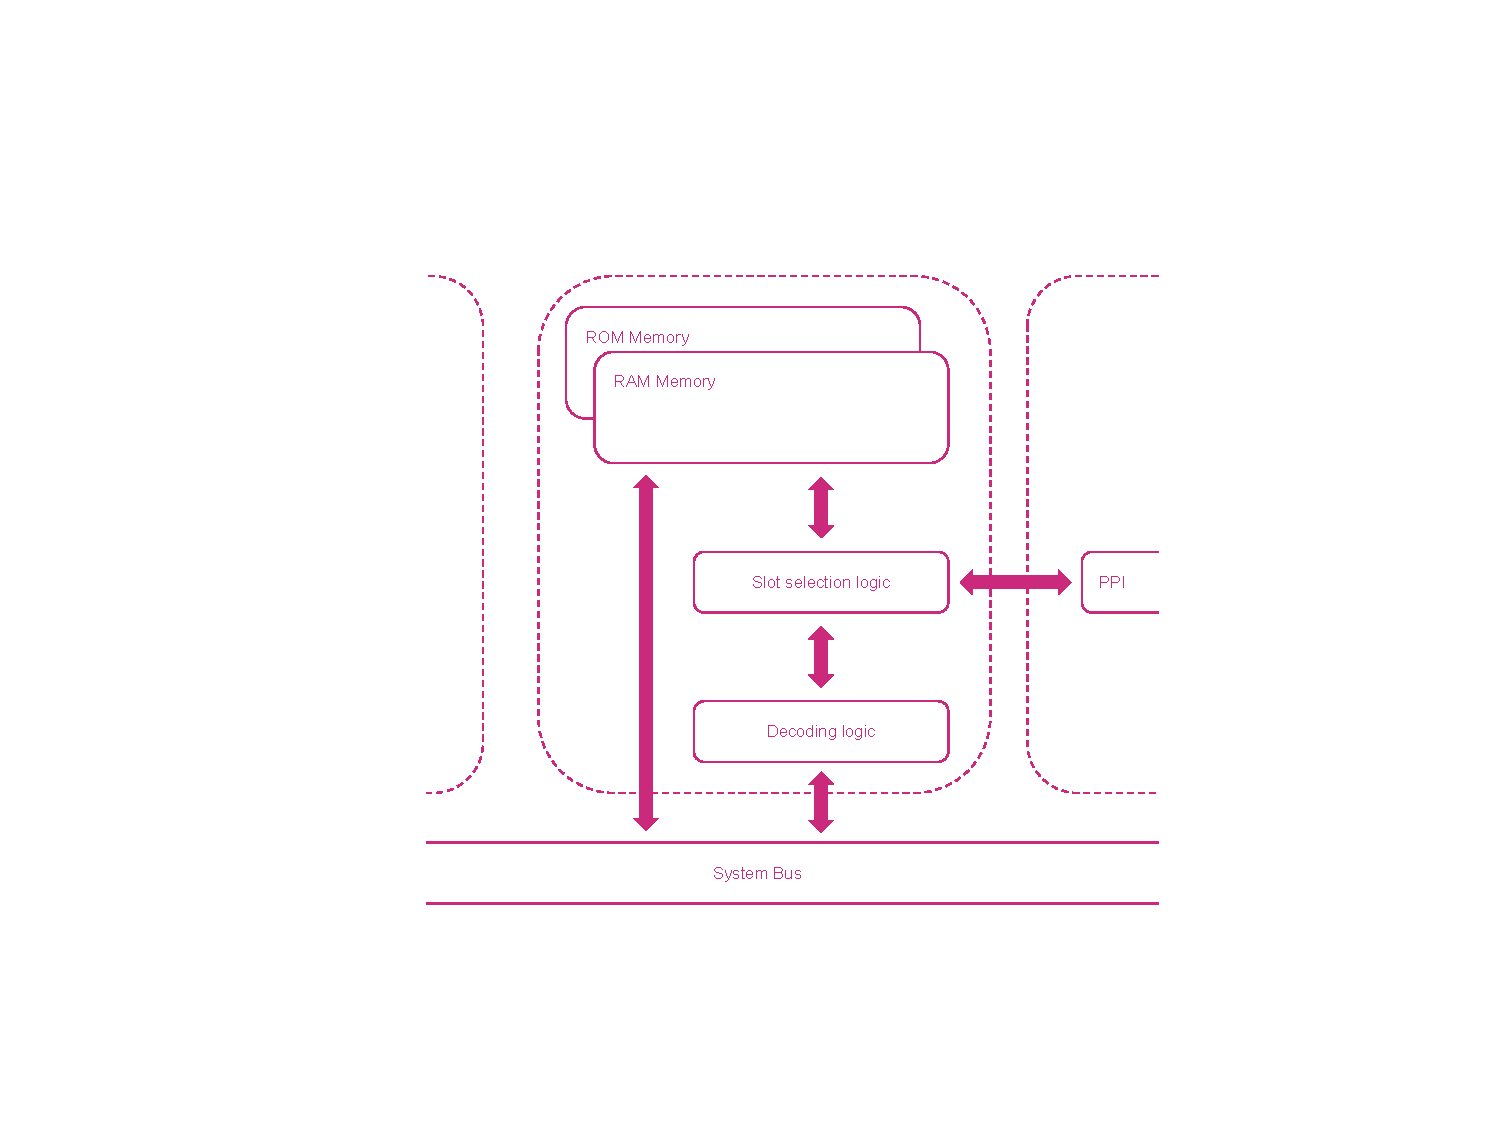
\includegraphics[width=1\linewidth,trim={0cm 100 0 100}]{images/figures/msx-arch-memory}
	\caption{High level architecture of the MSX memory}
	\label{fig:msx-arch-memory}
\end{figure}

\subsection{The Video Display Processor}

If we think about it, a computer made just of CPU and memory is a useless junk that only serves to dissipate heat and contribute to the global warming. It needs some peripherals to interact with the users, receiving data and programs as inputs and showing the result of these programs as outputs. \\

Perhaps the most important peripheral is the Video Display Processor (VDP). This is a circuit responsible of producing the video display in the computer. In the MSX standard, this is done by a chip of the Texas Instruments TMS9918 family, as shown in Figure \ref{fig:msx-arch-vdp}. This chip encapsulates all the logic necessary to display images in a TV set or suitable monitor. It is connected to the system bus through a decoding logic to adapt the signals. One of its main particularities is that it uses its own separated video RAM memory to store the images and the sprites it will display in the screen. \\

\begin{figure}
	\centering
	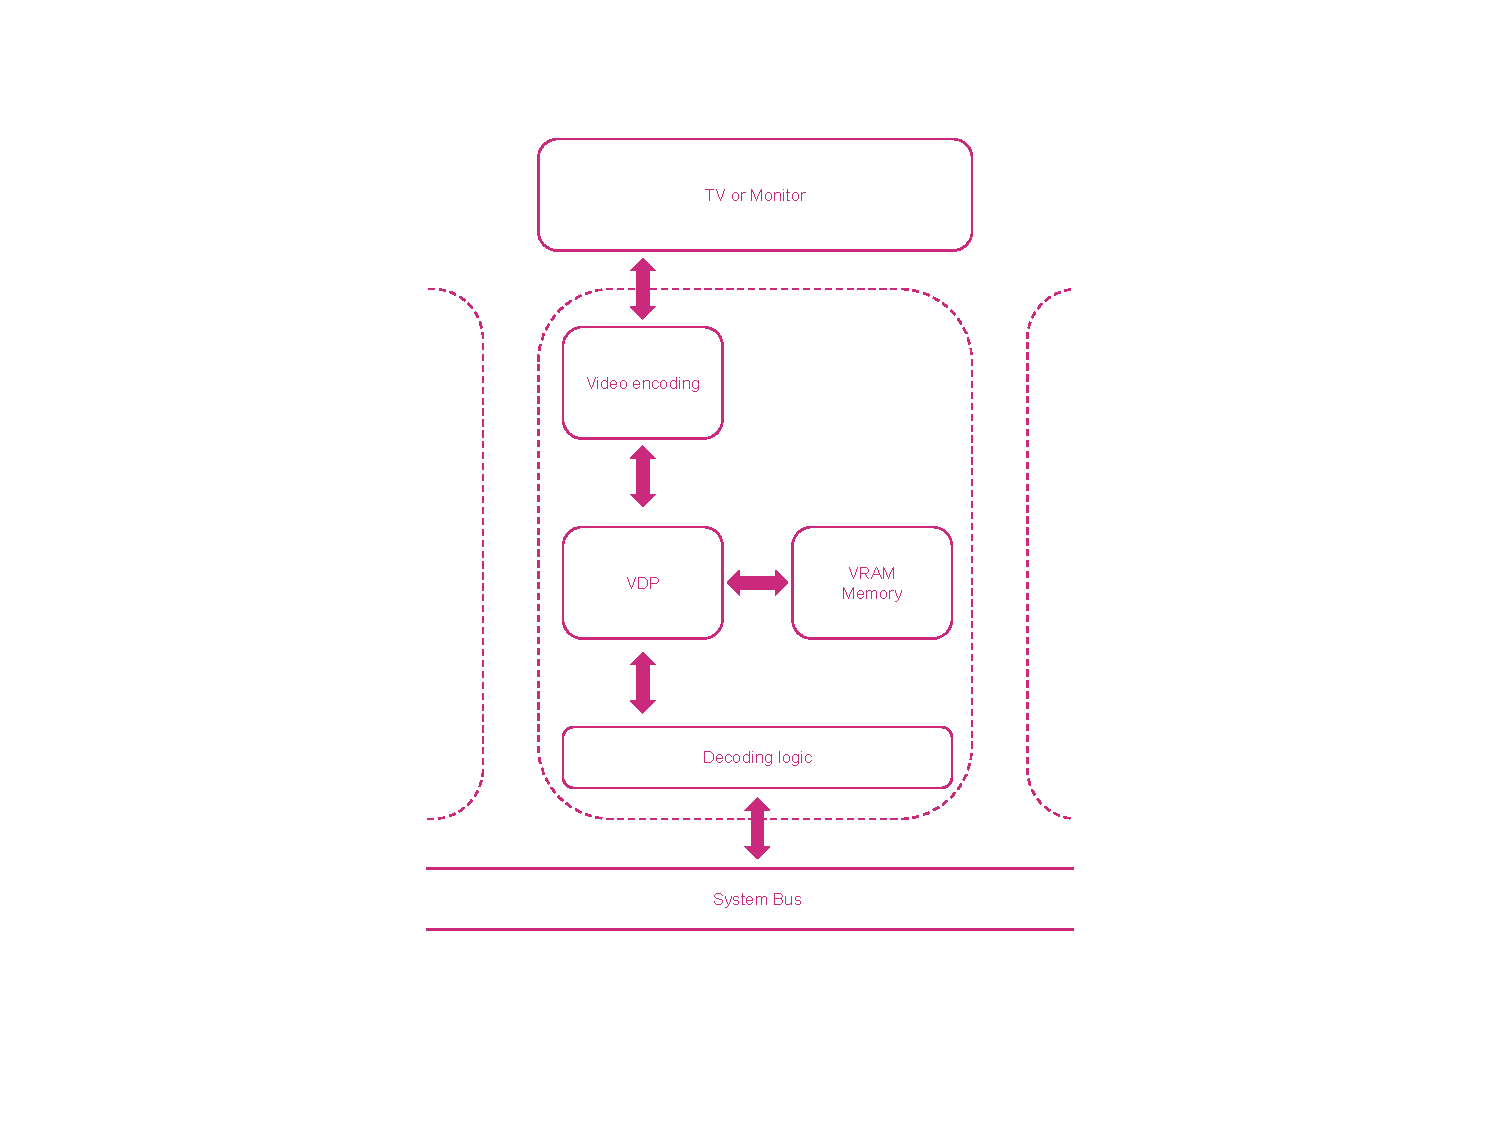
\includegraphics[width=1\linewidth,trim={0cm 100 0 100}]{images/figures/msx-arch-vdp}
	\caption{High level architecture of the MSX Video Display Processor}
	\label{fig:msx-arch-vdp}
\end{figure}

It is worth to remark this particularity of the VDP design in an MSX computer. Almost any other system uses a video display that shares the RAM memory with the CPU. The computer programs must write the data of the images they want to display into a specific section of the main RAM memory. And the display processor will read from that memory area to calculate the pixels that will be shown into the screen. \\

As you might think, sharing the memory between two different devices that can potentially access to the same addresses at the same time is not easy. This is known as memory contention. And it is full of tradeoffs. Consider that the video display cannot stop doing its job because the memory is being used by the CPU. If it does, we would observe artifacts in the screen such as flickering images caused by the interruption of the video stream. In some cases, this is addressed by finding the perfect timing on the accesses to the system bus, as Steve Wozniak did for the Apple ][. In some other cases, the CPU is forced to wait when memory contention occurs, losing precious CPU cycles and impacting the system performance. This is the case of the ZX Spectrum and the Amstrad CPC computers. \\

In contrast, the MSX computers strictly separates the system RAM from the video RAM. The programs only access the VRAM indirectly by sending \toref{I/O requests} to the VDP to perform read or write operations on the VRAM. The VDP coordinates the access to the memory for both: read the bitmaps to display the screen and process the read or write requests coming from the CPU. The result is a simpler computer architecture without memory contention that do not sacrifice CPU cycles. 

\begin{theory}{I/O requests}
	The Z80 microprocessor, as many others, includes the concept of I/O operations in its design. I/O is just an acronym of Input/Output. The CPUs that embrace this concept implement a specific way to communicate to and from system peripherals by means of an I/O request. \\\\
	
	An I/O request is a communication initiated by the CPU whose destination is a specific device attached to the system bus. The request can be one of two types: a read operation to transmit a byte from the device to the CPU, or a write operation to transmit a byte from the CPU to the device. The device that must respond to the request is identified by an 8-bit number known as the I/O port. The CPU uses the signals of the system bus to indicate the start of an I/O request, the port of the device that must respond, and whether it is a read or a write operation. The byte that is exchanged between the CPU and the device is also transferred throw the system bus. \\\\
	
	For example, if the CPU wants to write the byte 0xAB to the VRAM address 0x1234, it will have to follow this sequence of I/O requests:
	
	\begin{itemize}
		\item I/O request to port 0x99 to write the byte 0x34. This will tell the VDP the least significant bits of the VRAM address that will be written.
		\item I/O request to port 0x99 to write the byte 0x52. This is the six most significant bits of the VRAM address (0x12) that will be written, prefixed with 0b01. These two bits prefix indicates the VDP must be prepared for a VRAM write operation immediately after.
		\item I/O request to port 0x98 to write the byte 0xAB. This is the byte the VDP will write to VRAM address 0x1234.
	\end{itemize}
	
	Some other CPUs, such as the MOS 6502 or the Motorolla 68000 do not implement the concept of I/O request. These CPUs uses memory access instructions equally to access the memory or access other bus devices. This means part of the memory address space must be  reserved for I/O operations. 	
\end{theory}

\subsection{The parallel peripherals}

Once we can display the results of the programs our MSX computer executes, it is time to think about receiving some inputs. One of the most important pieces used in the MSX architecture to achieve this is the Parallel Peripheral Interface (PPI), shown in Figure \ref{fig:msx-arch-ppi}.\\

\begin{figure}
	\centering
	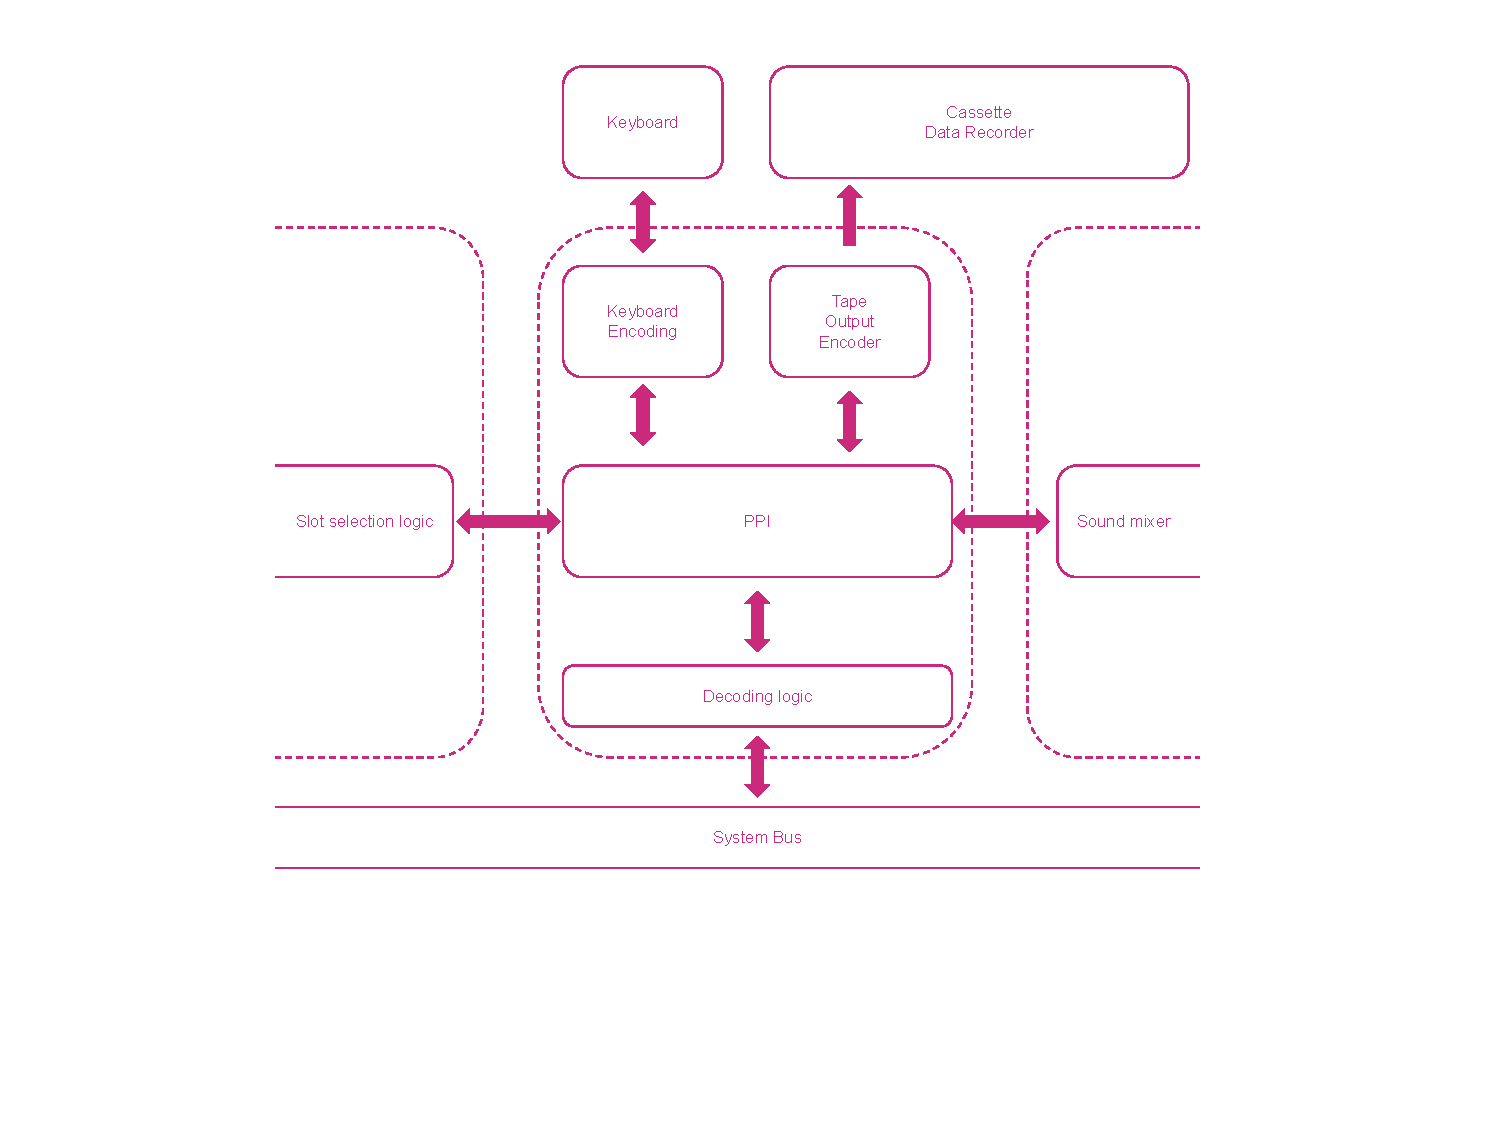
\includegraphics[width=1\linewidth,trim={0cm 100 0 100}]{images/figures/msx-arch-ppi}
	\caption{High level architecture of the MSX Parallel Peripheral Interface}
	\label{fig:msx-arch-ppi}
\end{figure}

The PPI is an Intel 8255 integrated circuit that will act as hardware controller for some peripherals and a few control lines of the system. This is the same chip included in the IBM PC computer, still present in the chipsets of most of modern PC designs. The 8255 has three 8-bit ports: A, B and C. Each port can be configured by software as input or output. The MSX BIOS will configure each port at convenience on system boot. \\

The system peripherals that are attached to the system through the PPI are connected by wires to some lines of its three ports, as shown in Figure \ref{fig:msx-arch-ppi-ports}. The mission of this chip in the MSX is to serve as an interface adapter for the peripherals that cannot be directly connected to the system bus, such as the keyboard and the cassette data recorder. Using I/O requests, the CPU can read from the input ports and write to the output ports of the PPI. Which is analogous to read or write from or to the peripherals attached to the ports.\\

\begin{figure}
	\centering
	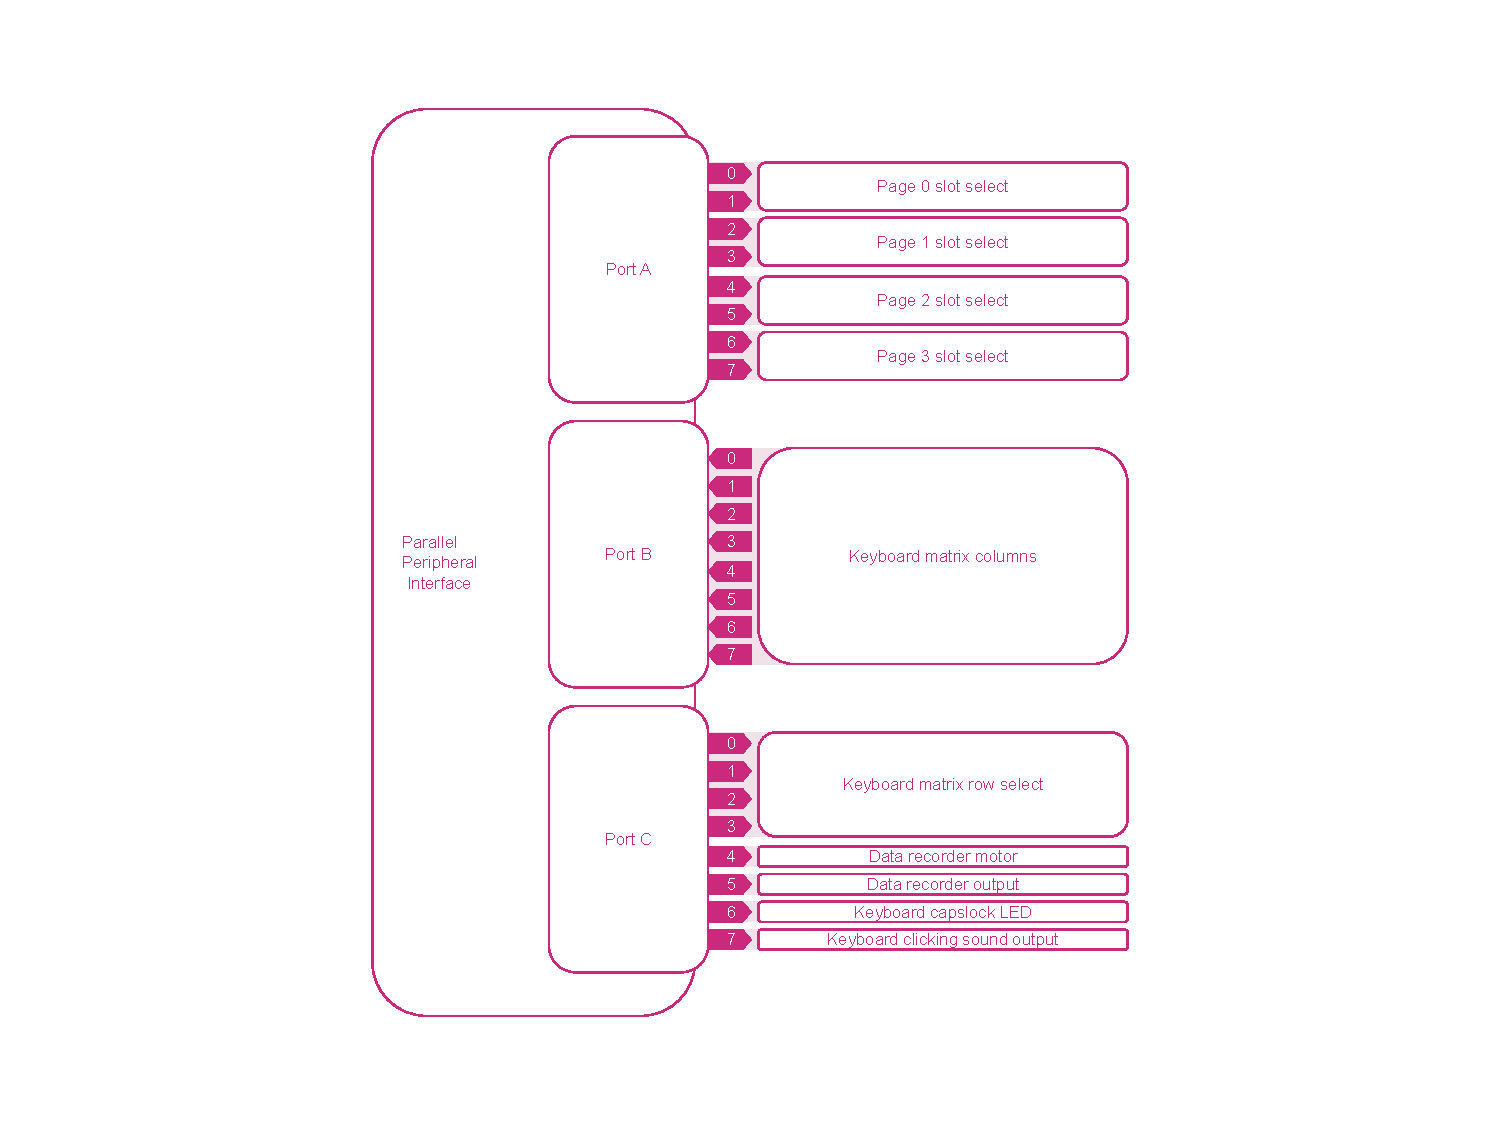
\includegraphics[width=1\linewidth,trim={0cm 50 0 50}]{images/figures/msx-arch-ppi-ports}
	\caption{Ports of the MSX Parallel Peripheral Interface}
	\label{fig:msx-arch-ppi-ports}
\end{figure}

The port A of the PPI is configured by the BIOS as output during the system boot. This port is responsible of choosing the memory slot to be used for every memory page. Each pair of bits determine the primary memory slot of a memory page. Since two bits are used per memory page, we can choose among 4 different primary memory slots. Do not panic if you still do not understand a word about this. It is a complex subject we will cover in detail later. \\

The port B of the PPI is configured by the BIOS as input. All eight bits are connected to the columns of the keyboard matrix. The port C is configured as ouput. The four less significant bits are used to select one row of the keyboard during the scanning process. Bits 4 and 5 are used to control the data recorder. Bit 6 is used to drive the LED of the capslock key of the keyboard and bit 7 is used to produce clicking sounds when keys are typed. \\

As you can see, the most important peripheral attached to the PPI is the keyboard. This is the time to tell how it works in an MSX computer and the meaning of these rows and columns thing. The keyboard of the MSX is implemented as a X-Y matrix of 8 columns and up to 12 rows, as shown in Figure \ref{fig:msx-arch-kbmatrix}. The total number of rows depends on the keyboard distribution. There is a key switch that connects every row to every column of the matrix. When a key is pressed, the row and the column connected by the switch form a closed circuit. When this happens, any current driven through the wire of the row will propagate to the column. Otherwise, if the key is not pressed, we will have an open circuit and the column will have no current. \\

\begin{figure}
	\centering
	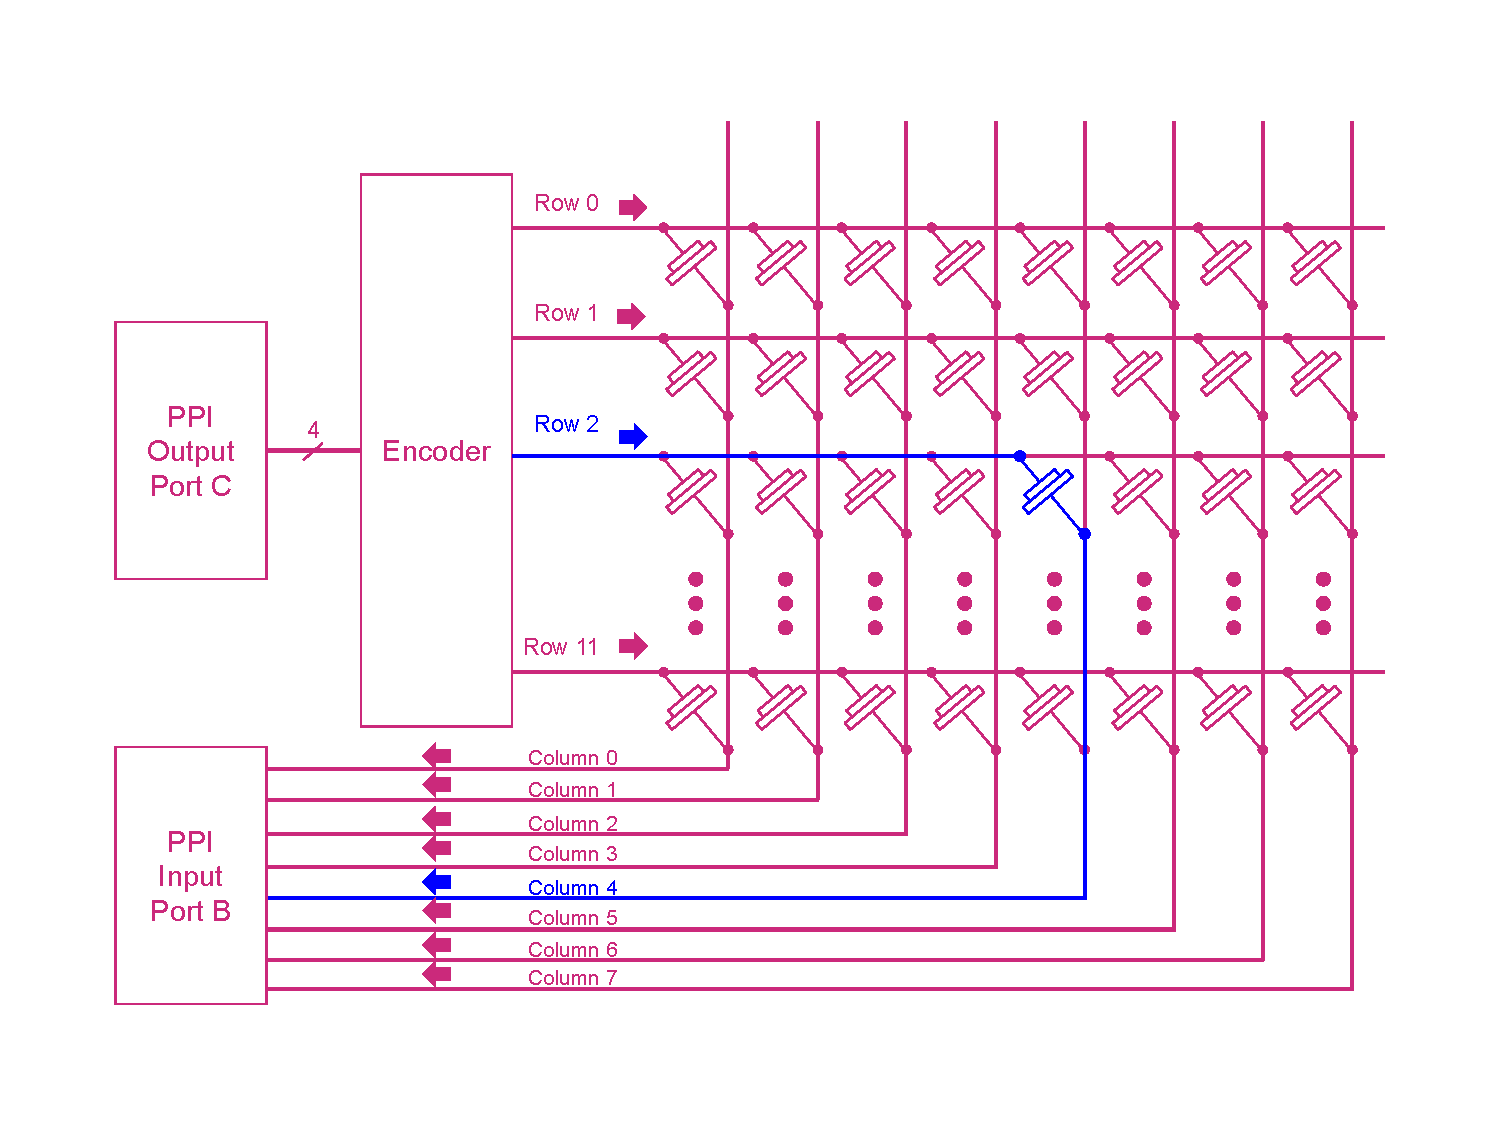
\includegraphics[width=1\linewidth,trim={0cm 5 0 0 40}]{images/figures/msx-arch-kbmatrix}
	\caption{Keyboard matrix of a MSX computer}
	\label{fig:msx-arch-kbmatrix}
\end{figure}

In order to make it work, the MSX uses the PPI to drive the row signals of the matrix and read the status of the columns.  The four less significant bits of output port C of the PPI are used to encode the row that will drive the current. And the whole eight bits of input port B are connected to the matrix columns. The system software, typically the BIOS, will scan the matrix periodically. On each scan, it will loop from the first to the last row. In each loop iteration, it will select the i-th matrix row and read the status of the 8 columns. The row can be selected by writing its 4-bit number in the corresponding bits of the port C of the PPI through an I/O request. The columns can be checked by reading the port B of the PPI through an I/O request. If that read of port C reveals the current is driven in the j-th column, it means the key located at i-th row and j-th column in the matrix is pressed. Otherwise, it is depressed. \\

The bit 6 of PPI port C is also involved in the keyboard operation. It drives the LED of the capslock key. As you might think, this is controlled by software. It can be turned on and off by setting 0 and 1 in that bit of port C, respectively. \\

The bits 4 and 5 of the PPI port C are connected to the cassette data recorder. The data recorder is an unexpensive storage device that uses cassette tapes to transmit information to and from the computer. It is a cassette player that reproduces the sounds from the tape when reading and records the sound signal on the tape when writing. The sound signals encode binary data in a special kind of frequency modulation known as FSK (Frequency-Shift Keying) following the Kansas City standard. This norm establishes that a “0” bit is encoded by one wave cycle at a frequency of 1200 Hz. While a “1” bit is encoded by two cycles of a 2400 Hz wave. The sound wave reproduces a sequence of beeps alternating between 1200 and 2400 Hz, which in fact represents zeroes and ones that are transmitted from or to the computer. \\

In the MSX, all this encoding is generated by software. The bit 5 of the PPI port C is used to generate a squared waveform when writing a file to the data recorder. This is made typically by the MSX BIOS by writing zeroes and ones in that bit of the PPI port one by one. Fortunately, this FSK encoding system operates at low frequencies, below 4800 Hz in the worst case. The Z80 processor at 3.58Mhz can write these sequences of bits fast enough to ensure the waveform is well formed. \\

The wave generated through bit 5 of PPI port C is squared because the signals of the PPI ports are digital. Thus, they can only generate +5 and 0 voltage levels, as shown in Figure \ref{fig:msx-arch-fskenc}. There is a tape output encoding circuit that transforms this squared wave into a sinusoidal waveform. Which is what the data recorder expects from the computer. The process to read a file is similar. But it involves other peripherals we will cover soon.

\begin{figure}
	\centering
	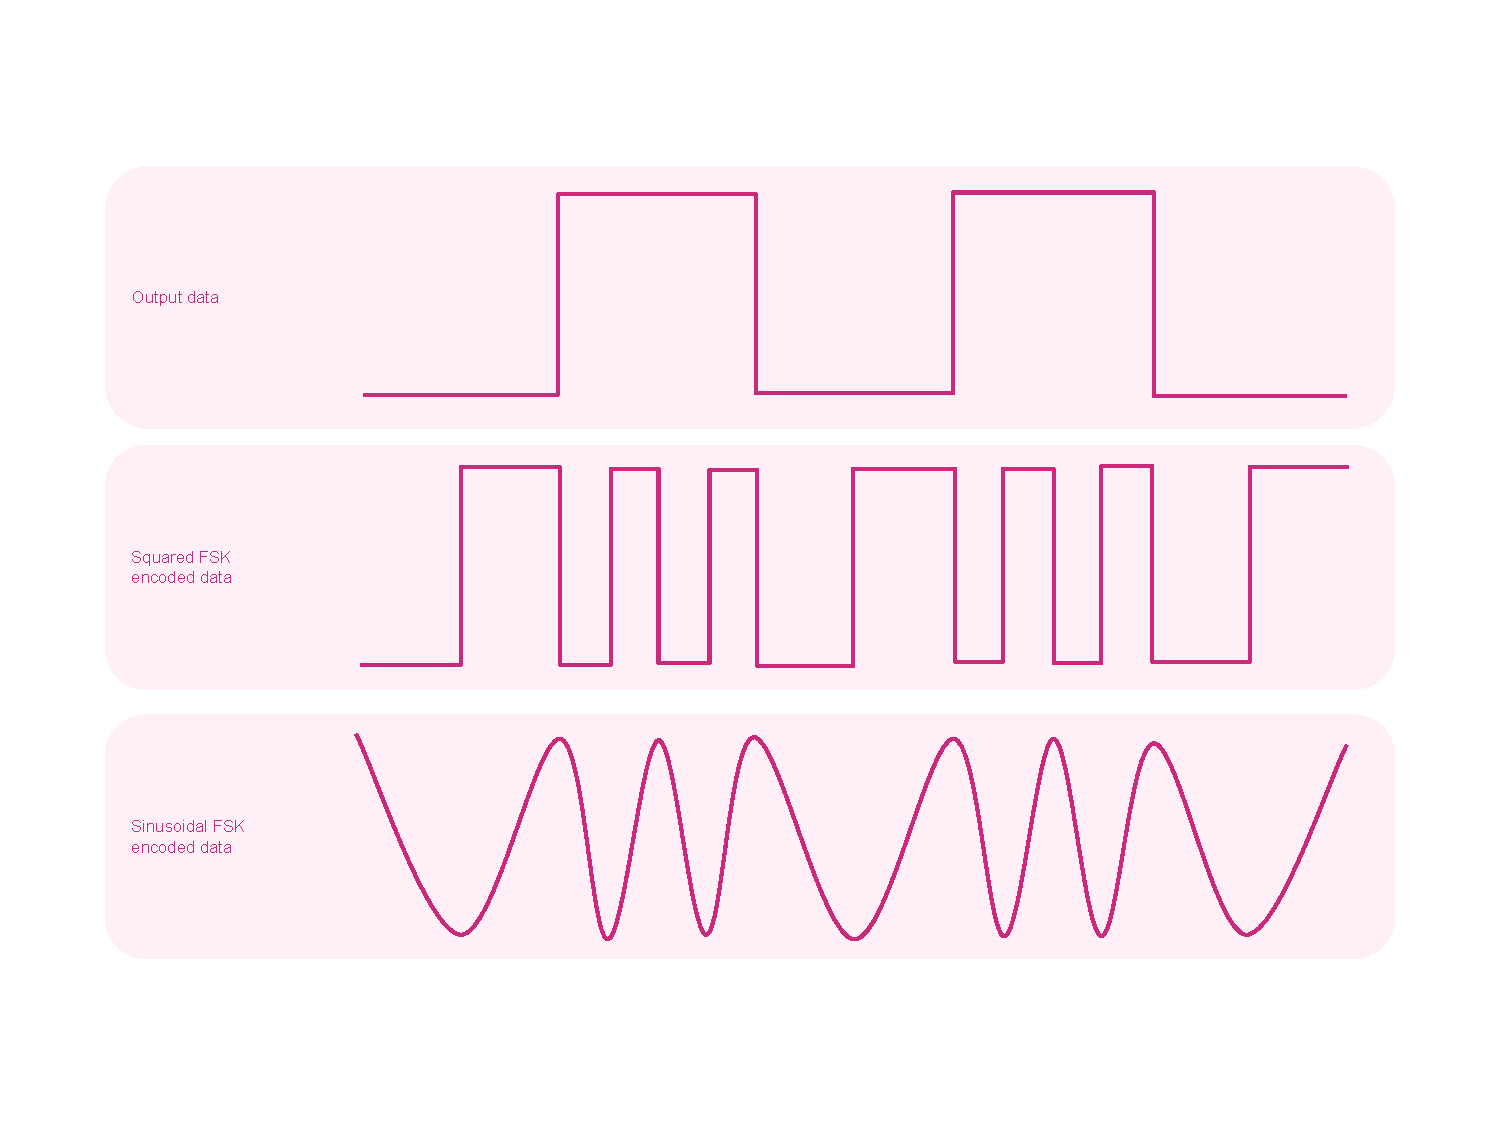
\includegraphics[width=1\linewidth,trim={0cm 80 0 80}]{images/figures/msx-arch-fskenc}
	\caption{FSK encoding in the MSX data recorder}
	\label{fig:msx-arch-fskenc}
\end{figure}

\subsection{Programmable Sound Generator}

A computer without a sound system is like a garden without flowers. And we already know the MSX is one of the best in its category. Of course, it has a programmable sound generator to play sounds and music. \\

This is implemented by the General Instrument AY-3-8910. This is a chip that can generate three independent sound channels programmed by software. It was released in 1978 and used in innumerable arcade machines and microcomputers. Including the ZX Spectrum, the Amstrad CPC and the Apple ][. \\

The 8910 is attached to the system bus of the MSX through a decoding logic to adapt its interface, as shown in Figure \ref{fig:msx-arch-psg}. Such interface give access to three different I/O ports: the address port, the data write port and the data read port. \\

\begin{figure}
	\centering
	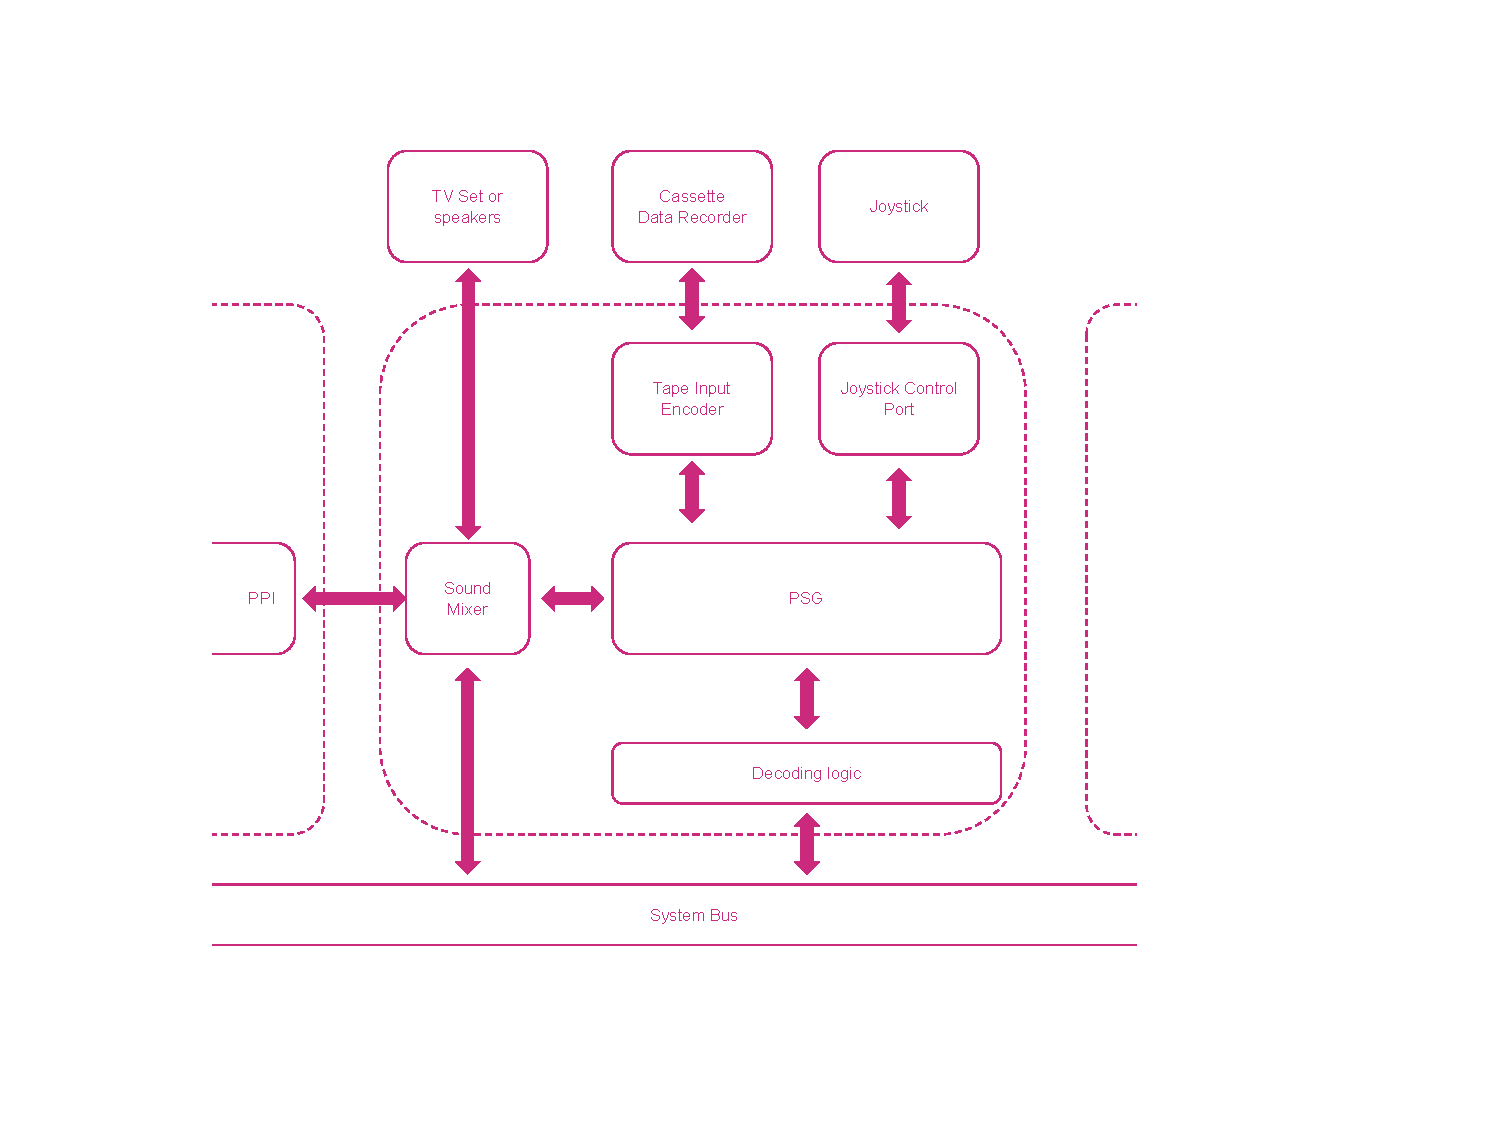
\includegraphics[width=1\linewidth,trim={0cm 80 0 50}]{images/figures/msx-arch-psg}
	\caption{High level architecture of the Programmable Sound Generator}
	\label{fig:msx-arch-psg}
\end{figure}

The address port is used to indicate the address of the internal register that will be read or written. The PSG has 16 internal registers numbered from 0 to 15. Writing the PSG register number in I/O port 0xA0 will prepare the chip to use that register in subsequent read or write operations.\\

The PSG data write port is available at I/O port 0xA1. This port is used to write bytes to the PSG register that was addressed by previous writes to 0xA0. The PSG data read port at 0xA2 does the same for reading. \\

Using these three ports, the system software can program the PSG to generate sounds. As said above, the PSG has three independent channels that can generate separated sounds. However, the MSX was designed in a time when the mono sound was the standard. Thus, the common choice of all MSX computers is to mix the three channels into a single sound signal. This is done by a sound mixer circuit. The mixer also receives the inputs from other devices that are also part of the final sound signal sent to the TV set or the speakers, as shown in Figure \ref{fig:msx-arch-psg}. \\

If you remember the Figure \ref{fig:msx-arch-ppi-ports}, the bit 7 of PPI port C is used to produce the characteristic click sound when the user types in the keyboard. This sounds comes from a rudimentary squared waveform produced by this bit from the PPI. The system software, typically the BIOS, will write an alternating sequence of zeroes and ones to this bit of the PPI port C that produces the squared wave. The port bit is connected to the sound mixer to include it in the sound signal that goes to the TV set or the speakers. \\

Finally, there is another input that feeds the sound mixer. It is the sound signal coming from the system bus. As we will see soon, the MSX is designed to be expandable. And to take this idea to the top, the external expansion devices can produce their own sound signal that will be mixed with those produced by the PSG and the keyboard clicks. Thanks to this, the PSG can be complemented with another sound chips connected through the expansion slots. \\

That is all concerning sound generation. However, the AY-3-8910 was designed to assume other tasks in the system. It also incorporates two I/O ports that can be used to connect parallel peripherals in a similar way as we do with the PPI. These ports are named A and B. They can be programmed as input or output. And in MSX, they are used to connect the general-purpose ports, the data recorder input and a few other IO/functions as shown in Figure \ref{fig:msx-arch-psg-ports}. \\

\begin{figure}
	\centering
	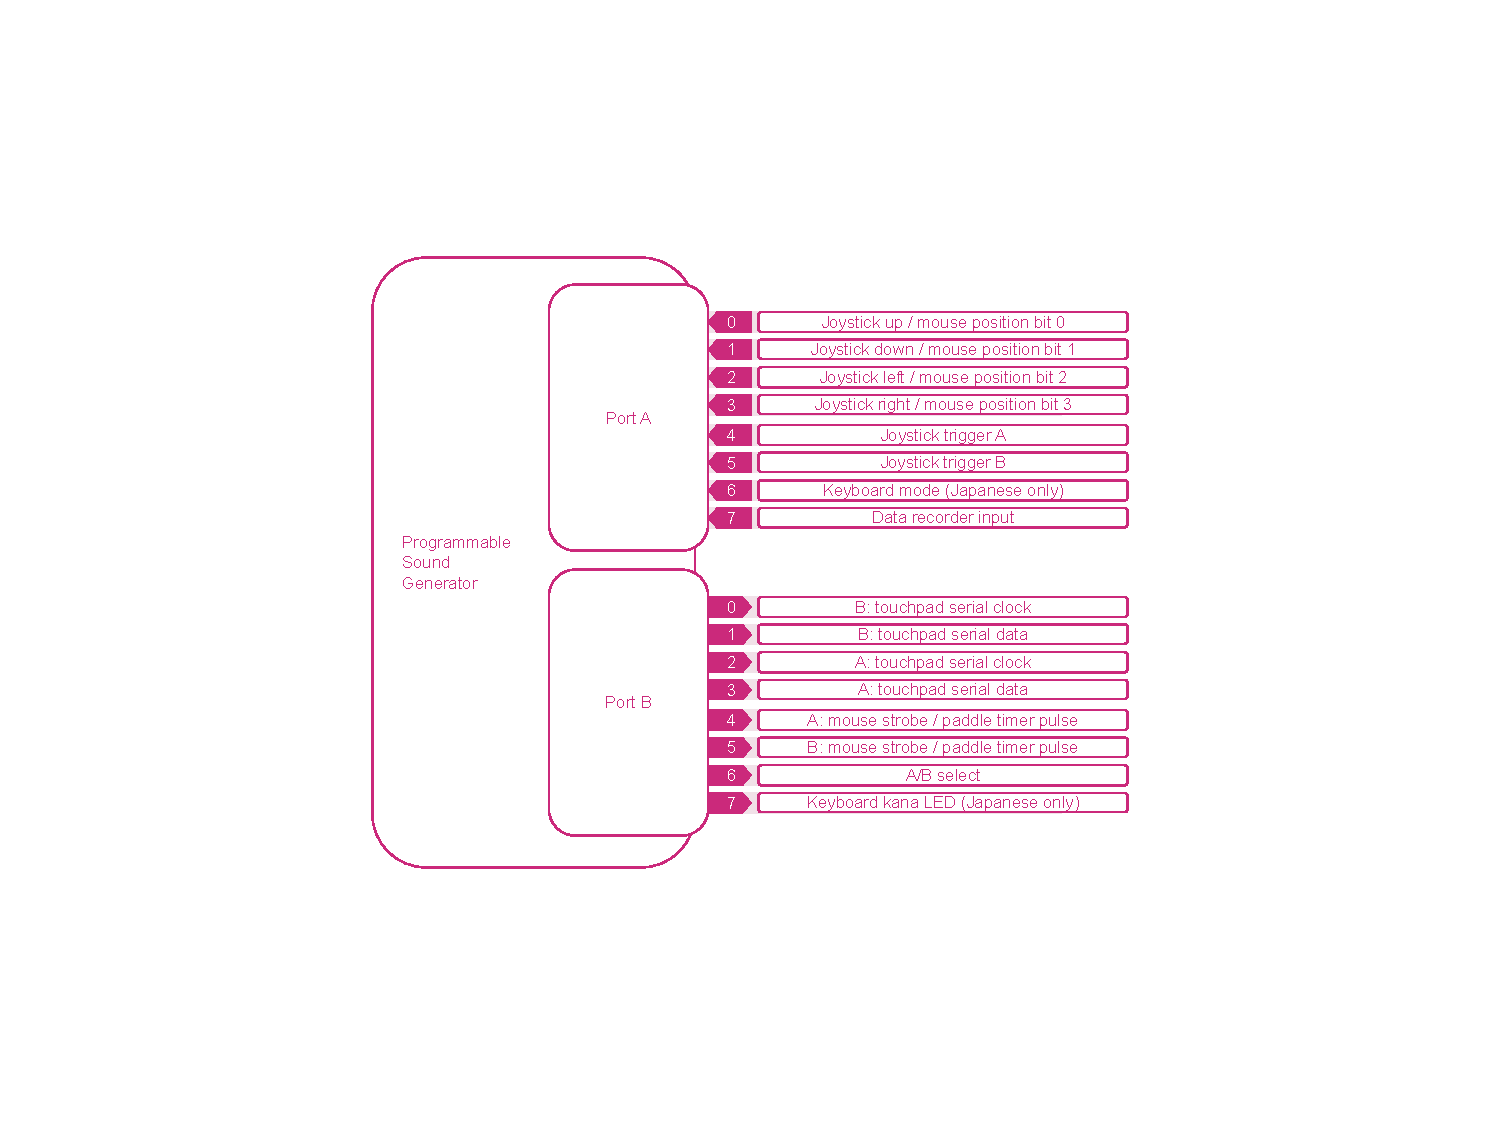
\includegraphics[width=1\linewidth,trim={0cm 120 0 100}]{images/figures/msx-arch-psg-ports}
	\caption{Ports of the MSX Programmable Sound Generator}
	\label{fig:msx-arch-psg-ports}
\end{figure}

The general-purpose ports are informally known as the joystick ports. This is because its main usage is to connect joysticks to the MSX. But they can be also used for many other device types such as mouses, trackpads, paddles, etc. \\

The port A of the PSG is configured as input by the MSX BIOS upon system boot. The four less significant bits are used to read joystick movements or mouse position values. The bits 4 and 5 are used to detect whether the trigger A and B is pressed or not, respectively. The bit 6 is used in Japanese MSX models only. It tells what kind of key distribution the computer has, where 1 is JIS and 0 is ANSI. The bit 7 is used to receive the input signal from the data recorder. \\

As we have seen before, the data recorder produces a sound signal that is directly connected to the computer. As shown in Figure \ref{fig:msx-arch-psg}, this analog sound signal is converted into a digital equivalent that can be received in the bit 7 of PSG port A. \\

The port B of the PSG is configured as output by the MSX BIOS upon system boot. The four less significant bits are used for touchpad devices only to transmit the clock and data signals. For the rest of devices, they will be set to 1. The bit 4 and 5 are the mouse strobe signal or the paddle timer pulses for devices plugged to connector A and B, respectively. The bit 6 is the connector select bit. Did you wonder what device the six less significant bits from port A refer to? Yes, as we can have two joysticks, mouses, etc., it should be possible to read movements from two different devices. The fact is that these six bits from port A are multiplexed. It means the same wires are used to carry the movement information from connector A or B. The bit 6 of port B determines which device will put their information on the wires that connect to PSG port A. Finally, the bit 7 drives the LED of the Kana key in Japanese keyboards.

\subsection{Expansion slots}

We are almost done. There is only one more important part of an MSX system to discuss: the expansion slots. \\

As mentioned above, the MSX system was designed with the expansibility in mind. The intention of its authors was to allow the users to add new hardware and increase the capacity of their computers as easily as possible. To achieve this, they designed the computer to have expansion slots. \\

You are probably more than used to use expansion slots, also commonly known as cartridge slots. They are 50 pin edge connectors in the motherboard of the MSX where the user can insert cartridges to expand the system. These cartridges are RAM expansions, games, storage devices, floppy drives, sound chips, etc. MSX systems have at least one cartridge slot, but it is not unusual to see models with two slots. In some other cases a cartridge slot is complemented with a 50-pin expansion IDC connector that has the same or similar pinout. The popular Spectravideo SVI-728 is an example of this. \\

The expansibility of the cartridge slot is possible because, in essence, the slot connector is an extension of the system bus, as shown in Figure \ref{fig:msx-arch-slots}. Most of the lines that comprise the system bus are included in the 50 pins connector. Thus, connecting a cartridge to the slot is equivalent to having such hardware soldered into the motherboard of the computer.

\begin{figure}
	\centering
	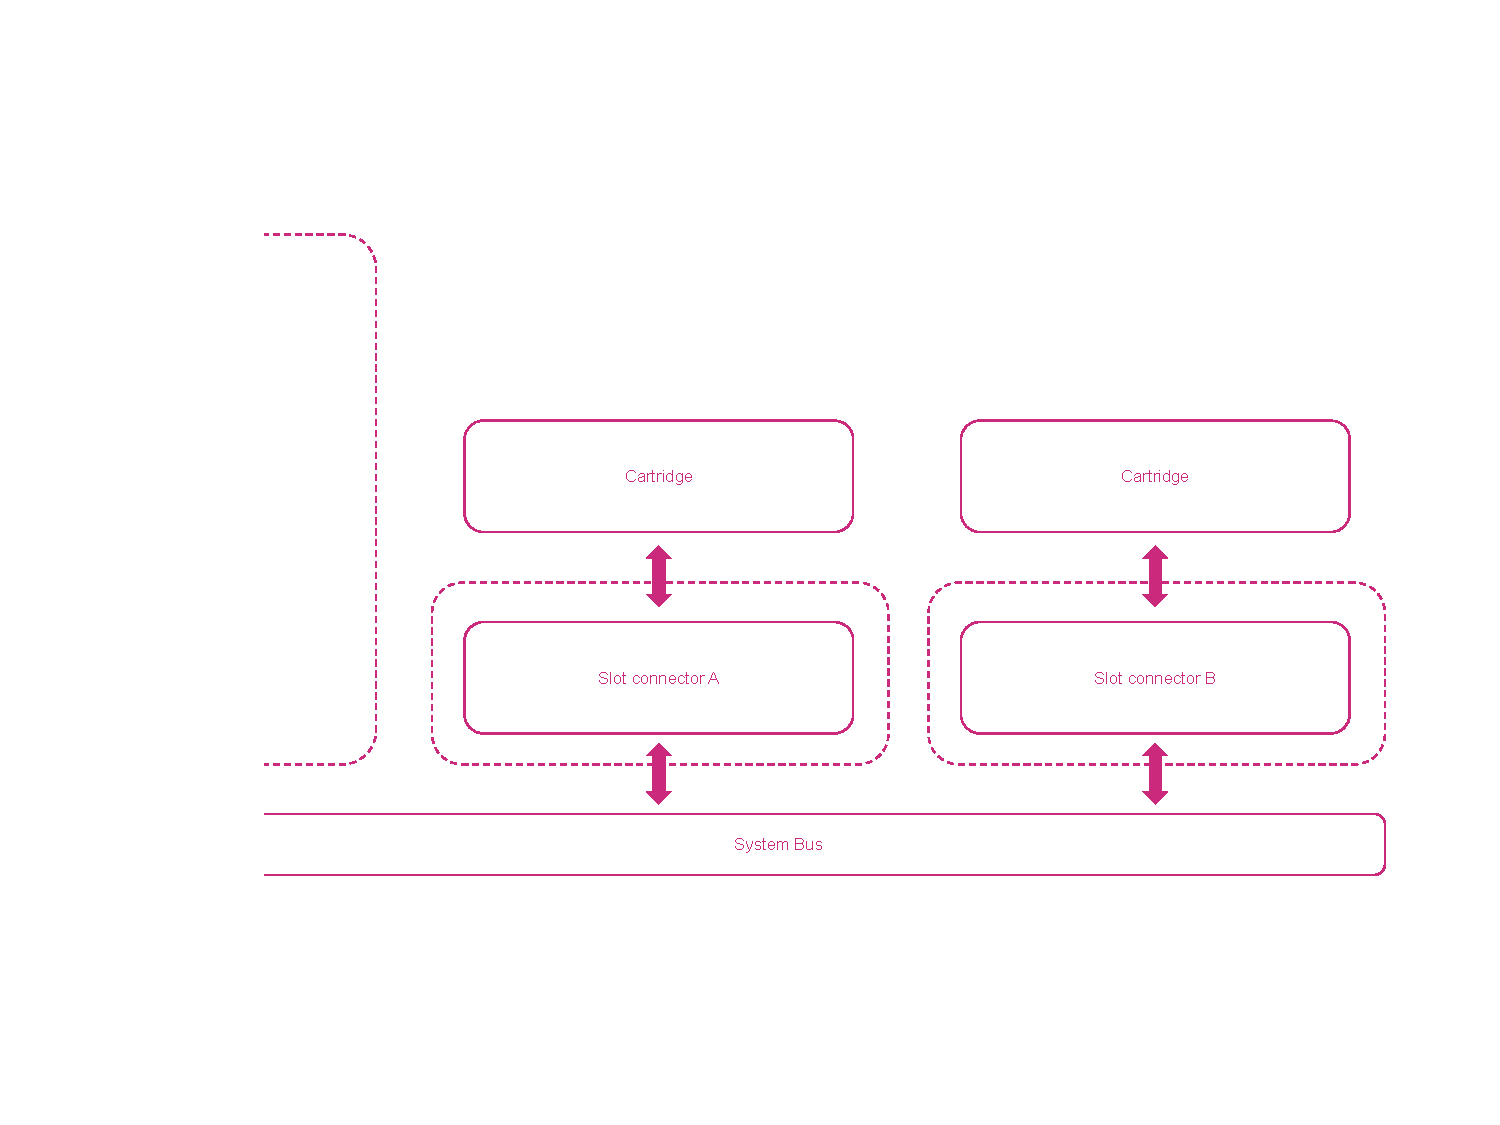
\includegraphics[width=1\linewidth,trim={0cm 120 0 100}]{images/figures/msx-arch-slots}
	\caption{High level architecture of expansion slots in a MSX Computer}
	\label{fig:msx-arch-slots}
\end{figure}

\subsection{Summary}

We have seen an overview of the most important parts that conform an MSX system. There are some others that will not be covered here, such as the serial communications port or the printer port. \\

As you can see, and as we revealed at the beginning of this chapter, the architecture of the MSX computer is extremely simple. Compared to other contemporary computers such as the IBM PC, the MSX do not have neither an interrupt nor a DMA controller. It has no mass storage device other than the data recorder and it has no real-time clock. Most of its hardware is based on off-the-shelf components, such as the TMS9918 VDP or the AY-3-8910 PSG. This contrasts with other hardware platforms such as the ZX Spectrum, the Amstrad CPC or even the IBM PC, which mount their own proprietary video display controllers. The MSX was designed to be cost-effective and standard. And this means a simple architecture easy to reproduce. \\

As we have seen from the beginning of this chapter, the most complex part of the MSX architecture is the memory system. Due to its relevance, we will dedicate a whole section to it.

\section{MSX Memory Slots}
\label{sec:msx-mem-slots}

\subsection{Bank switching}

The Z80 microprocessor uses 16-bit numbers to represent memory addresses. This means it can reference 65,536 memory locations. Assuming each memory location is 8-bit size, the whole memory space has 64KB. \\

In the time when the Z80 CPU was designed, that memory was enough for almost any purpose. But as the computers acquired more power and the user demands increased, the needs for more and more memory also appeared. In 1984, when MSX architecture was set, most computer engineers were incorporating in their designs methods to break the 64KB barrier present in most CPUs. These methods are based on what is known as memory {\bf bank switching}. \\

The concept is simple, although the implementation may become cumbersome. Instead of having a single RAM memory region, we will have multiple. Each region will be called a bank. The system determines what memory bank is used by the CPU in each instant in function of some programmable configuration and the memory address that is being used. \\

For example, a Z80-based computer can have four banks of 64KB of RAM memory each. If we put them all together, they are 256KB of memory, as shown in Figure \ref{fig:msx-mem-banks}. That is indeed not bad for an 8-bit computer. The software can choose what bank is active using a 2-bit register that is accessible through I/O requests. In this example the two bits could be part of the port of a PPI or similar, as we have seen at the beginning of this chapter. The system BIOS can preconfigure this bank select register with the value 0b00 so the first 64KBs of memory are visible to the CPU. At some point, the program can write the value 0b01 to the bank select register to switch to the memory bank 1. This means the CPU will see after this the memory from 64KB to 128KB. With bank 0b10 and 0b11, the memory segments from 128KB to 196KB, and from 196KB to 256KB, respectively will be visible to the CPU. \\

\begin{figure}
	\centering
	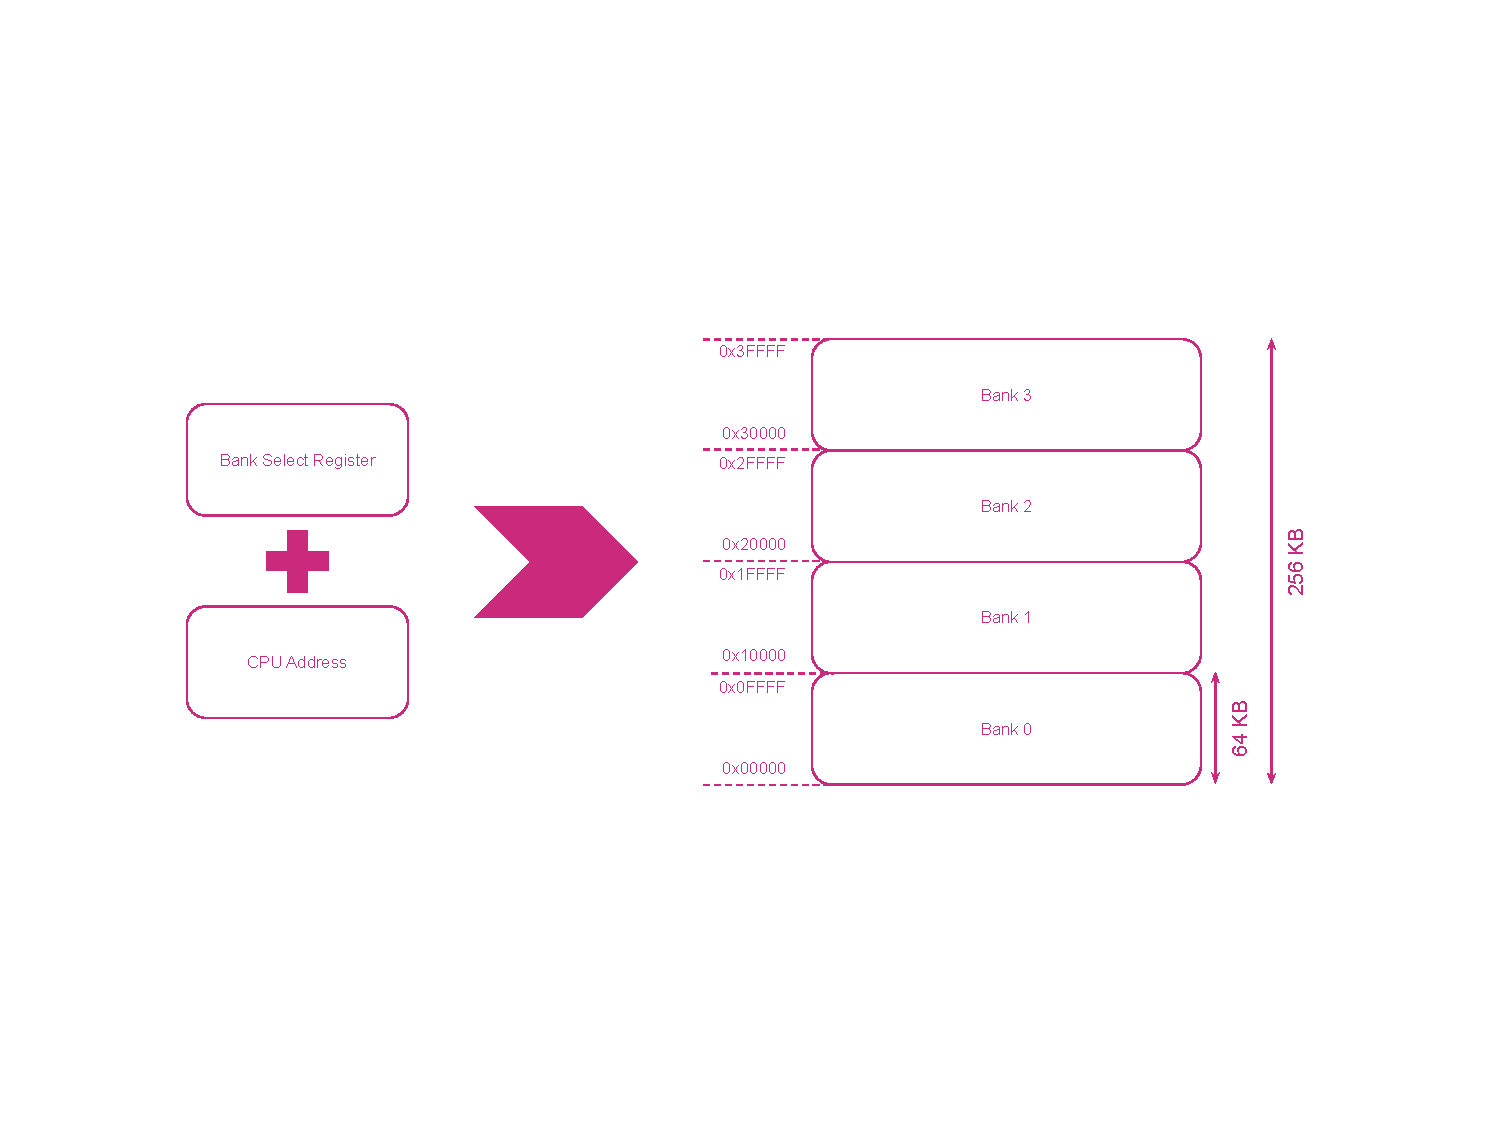
\includegraphics[width=1\linewidth,trim={0cm 150 0 100}]{images/figures/msx-mem-banks}
	\caption{An example of memory bank switching}
	\label{fig:msx-mem-banks}
\end{figure}

If you think about this in terms of memory addresses, you will note we are extending the memory addresses from 16 bits to 18 bits. To distinguish both, we may call the 16-bit address generated by the CPU as logical address and the extended 18-bit address as physical address. The physical address results from concatenating the contents of the bank select register to the logical address. Thus, if bank 2 is selected and the CPU requests an access to the memory location at 0x800A, the physical address will be 0x2800A (0x2 concatenated to 0x800A). \\

Unfortunately, this bank switch solution is too naïve and will not work in the real world. This is because we are considering the whole memory space is switched when a new bank is selected. And this interrupts the execution of the program. \\

For example, consider a program located at logical address 0x8000 is running with the bank 0 active. This is the physical address 0x08000. At some point, the program decides it needs more memory, so it must switch to the bank 1. After the switch, the memory seen by the CPU at logical address 0x8000 is no longer at physical address 0x08000, but 0x18000. In other words, the program the CPU was executing suddenly disappears. The next instruction the CPU will execute after bank switching is in 0x18000 region of physical memory, which contains uninitialized memory. \\

As we already mentioned above, this is typically addressed by also considering the segment of the memory that is being addressed as an input to calculate the memory bank. We can extend our example such as instead of having one bank select register, we have four of them. The first register will indicate the bank of memory space located from logical address 0x0000 to 0x3FFF. The second one is the bank for logical addresses between 0x4000 to 0x7FFF. And the third and fourth bank registers will be used for the logical address space from 0x8000 to 0xBFFF and 0xC000 to 0xFFFF, respectively. \\

In the case of a program that is located at physical address 0x08000, the 3rd bank select register will have a value of 0. The rest of register can have any other values, pointing to the same bank or another. If the program decides to make use of more memory, it can switch the 1st, 2nd and 4th bank registers to point to new banks with available memory. But it must not change the 3rd register or the program will suddenly disappear as we have seen before. 

\subsection{MSX Slots}

Although you may find this surprising (or not), what we had described above are the basics of what the MSX system does with its memory.\\

The MSX divides the 64 KB of the logical address space of the Z80 CPU by four. Each logical address space segment is called a page. The pages are shown in Table \ref{table:msx-mem-pages}.

\begin{table}[h]
	\centering
	\begin{tabular}{r|l|l}
		{\bf Page} & {\bf Start logical address} & {\bf End logical address} \\
		0          & 0x0000                      & 0x3FFF                    \\
		1          & 0x4000                      & 0x7FFF                    \\
		2          & 0x8000                      & 0xBFFF                    \\
		3          & 0xC000                      & 0xFFFF                    \\
	\end{tabular}
	\caption{MSX memory pages}
	\label{table:msx-mem-pages}
\end{table}

The physical memory region that is mapped to each page is called a slot. There are four primary slots, and each of them can be extended by another four secondary slots to a total maximum of 16 slots. But we will cover this later. \\

The primary slot configured for each page is determined by the port A of the PPI, as we have seen before. Each pair of bits of that port provide a number from 0 to 3 that tells what slot is used by that page, as we seen in Figure \ref{fig:msx-arch-ppi}. The slots can be reconfigured with I/O write requests to the PPI to switch the bits of the port A. \\

That is to configure the slots for each memory page. But what is exactly a slot? In the previous section, we have simplified the example by telling each bank is a 64KB region of RAM memory. But the real life is more complicated. In the real world, we have RAM and ROM memories. And in the case of the MSX, we want to have an extensible system. And that includes adding cartridges with RAM expansion or some hardware that has BIOS extensions written in ROM memories to manage the device. That is why in MSX we talk about slots, and not banks. \\

An MSX slot is anything that can respond to memory read and write operations. Typically, an MSX system has some built-in slots with some RAM or ROM memory. While some other slots are provided by… do you guess? Yes! The cartridge slots! \\

We had said the cartridge slots are expansions of the system bus. And they are indeed! But each cartridge slot has a designated memory slot. The 50-pin connector incorporates a select signal activated when it is targeted as the active slot when some page is addressed. When this happens, the cartridge connected to the slot must respond to the memory operations when they occur.\\

An example of this slot organization is shown in Figure \ref{fig:msx-mem-slotsprim}. In this case, the system has two built-in primary slots. The slot 0 contains a ROM memory from address 0x0000 to 0x7FFF. This ROM memory contains the MSX-BIOS and the MSX-BASIC in pages 0 and 1, respectively. Pages 2 and 3 are not wired. The slot 1 is a 64KB RAM memory occupying the for pages. The slots 2 and 3 are connected to the cartridge slots of the computer. In this example, we see a floppy drive connected to the cartridge slot A, which is the memory slot 2. This cartridge contains a ROM memory with an MSX-DISK BIOS extension to manage the floppy drive at memory page 1. In the cartridge slot B, which is the memory slot 3, we had plugged the popular game Arkanoid. This cartridge contains a ROM located at pages 1 and 2 with the game program and data. \\

\begin{figure}
	\centering
	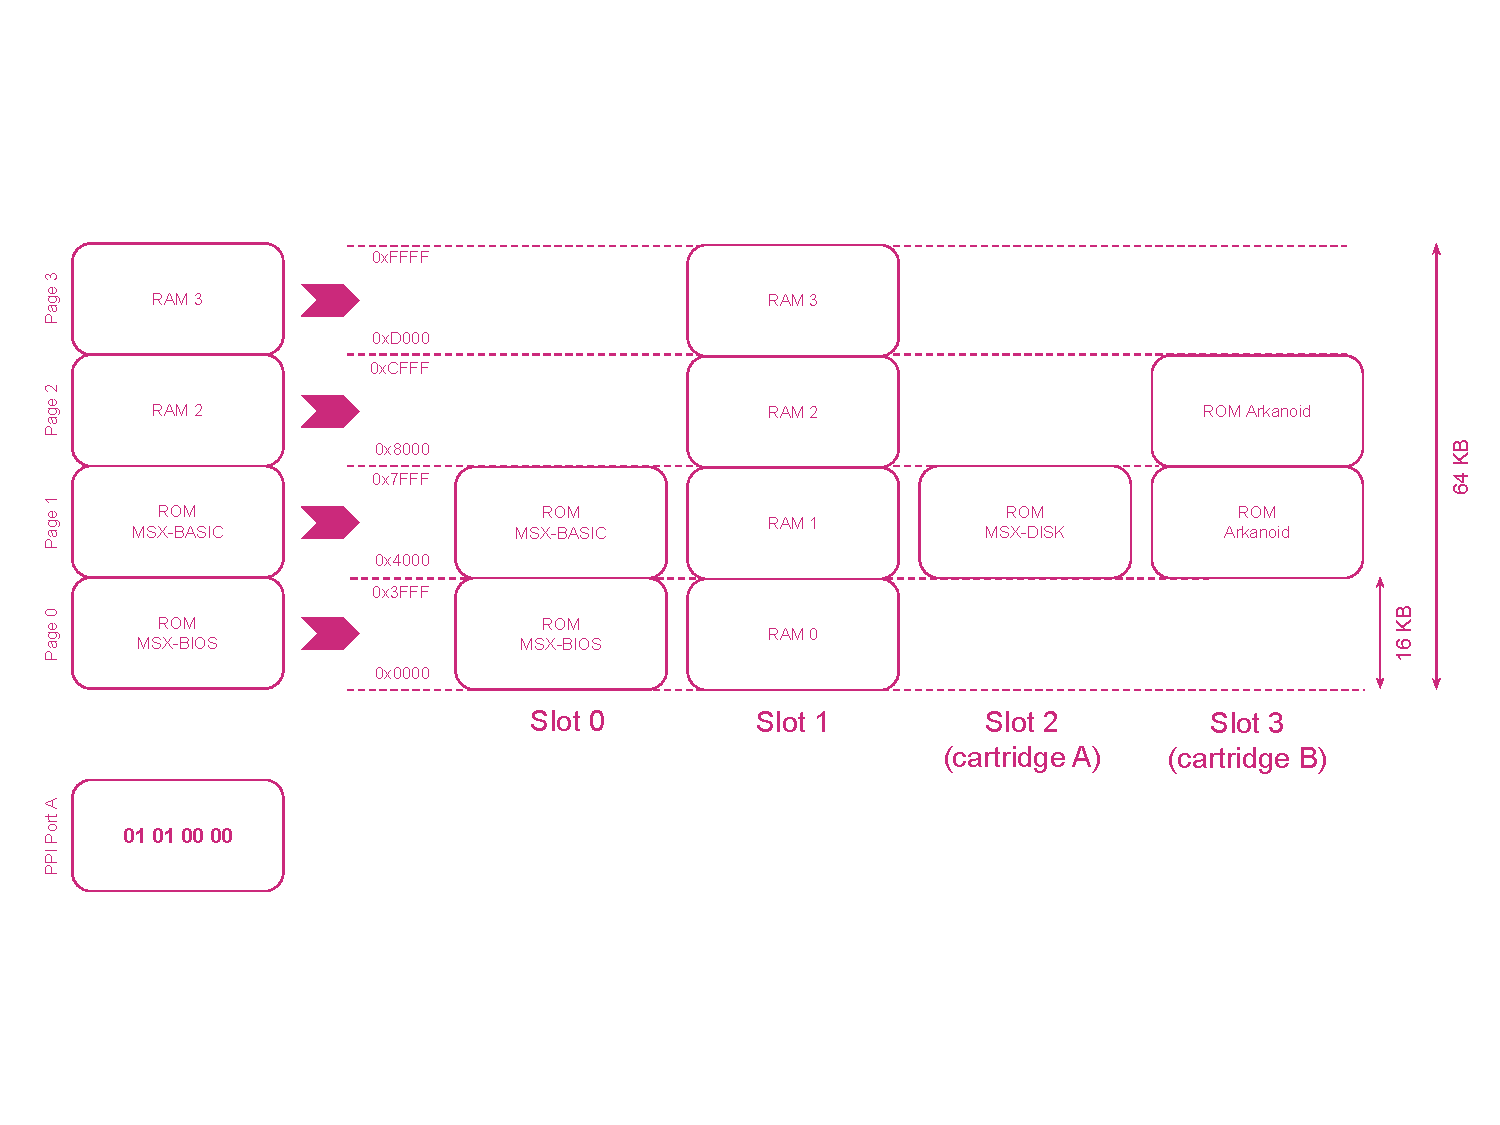
\includegraphics[width=1\linewidth,trim={0cm 100 0 80}]{images/figures/msx-mem-slotsprim}
	\caption{MSX memory slots configuration}
	\label{fig:msx-mem-slotsprim}
\end{figure}

In this example, the PPI port A is set to 0b01010000. This means the page 0 and 1 are mapped to the slot 0. That is why the MSX-BIOS and the MSX-BASIC are visible to the CPU. The page 2 and 3 are mapped to the slot 1. This is the slot full of RAM memory. Thus, the CPU will see RAM memory in the two upper pages. \\

Now let us say we load a program from the data recorder to the RAM at page 2 and run it. The code of the program can determine it needs more RAM than the 32KB already mapped. In order to use more RAM, it can configure the RAM slot in the page 1 by writing 0b01010100 to the PPI port A. Thus, it gets rid of the MSX-BASIC code to increase the RAM to 48KB. If the program needs even more RAM, it can configure the slot 1 for page 0 as well, such that the whole address space is full of RAM. \\

Please note the slot reconfiguration is not irreversible. Even in the case the program needs the whole 64KB of RAM memory, it does not mean it cannot use the MSX-BIOS anymore. For example, it might configure page 0 to use the RAM slot only when it must read or write to it. And once finished, restore the slot configuration to have again the MSX-BIOS code in the page 0. The same principle applies to any other memory page. There is only one restriction in this model: you cannot change the slot of the page where the current program is running. Because as we have seen before, this will interrupt the program. \\

One important note: the slot distribution seen here is just an example. The MSX standard does not indicate any specific memory layout. Some vendors decide to use the slot 1 for RAM. Some others use the slot 3. And they put the cartridges in slots 1 and 2. Some others only have 1 cartridge slot, so one of the memory slots is not used. Each vendor decides their own slot distribution. The software or the users must not make assumptions on where each memory device is located. Such assumptions had caused historical incompatibilities by some software that do not run properly on any MSX computer.

\subsection{Secondary memory slots}

Finally, it is time to discuss about the expanded slots. We already mentioned that each slot can be expanded such that it can contain four secondary slots. It means this slot will respond to read and write operations by forwarding the request to another sub-slot. The MSX standard specifies a way to configure the sub-slot that will attend the memory accesses when the primary slot is selected in the PPI. This is with a register located in the address 0xFFFF of the primary slot. This register operates in the same way as the port A of the PPI, with each pair of 2 bits selecting the sub-slot that will be used for each memory page. \\

Let us see this with an example, shown in Figure \ref{fig:msx-mem-slotssec}. Some MSX system may have the slot 1 expanded with two sub-slots. The sub-slot 0 contains 4 pages of RAM. The sub-slot 1 contains one page of ROM with some MSX-BIOS expansion. This primary slot 1 has a hardware register that responds to read and write operations at the address 0xFFFF. \\

\begin{figure}
	\centering
	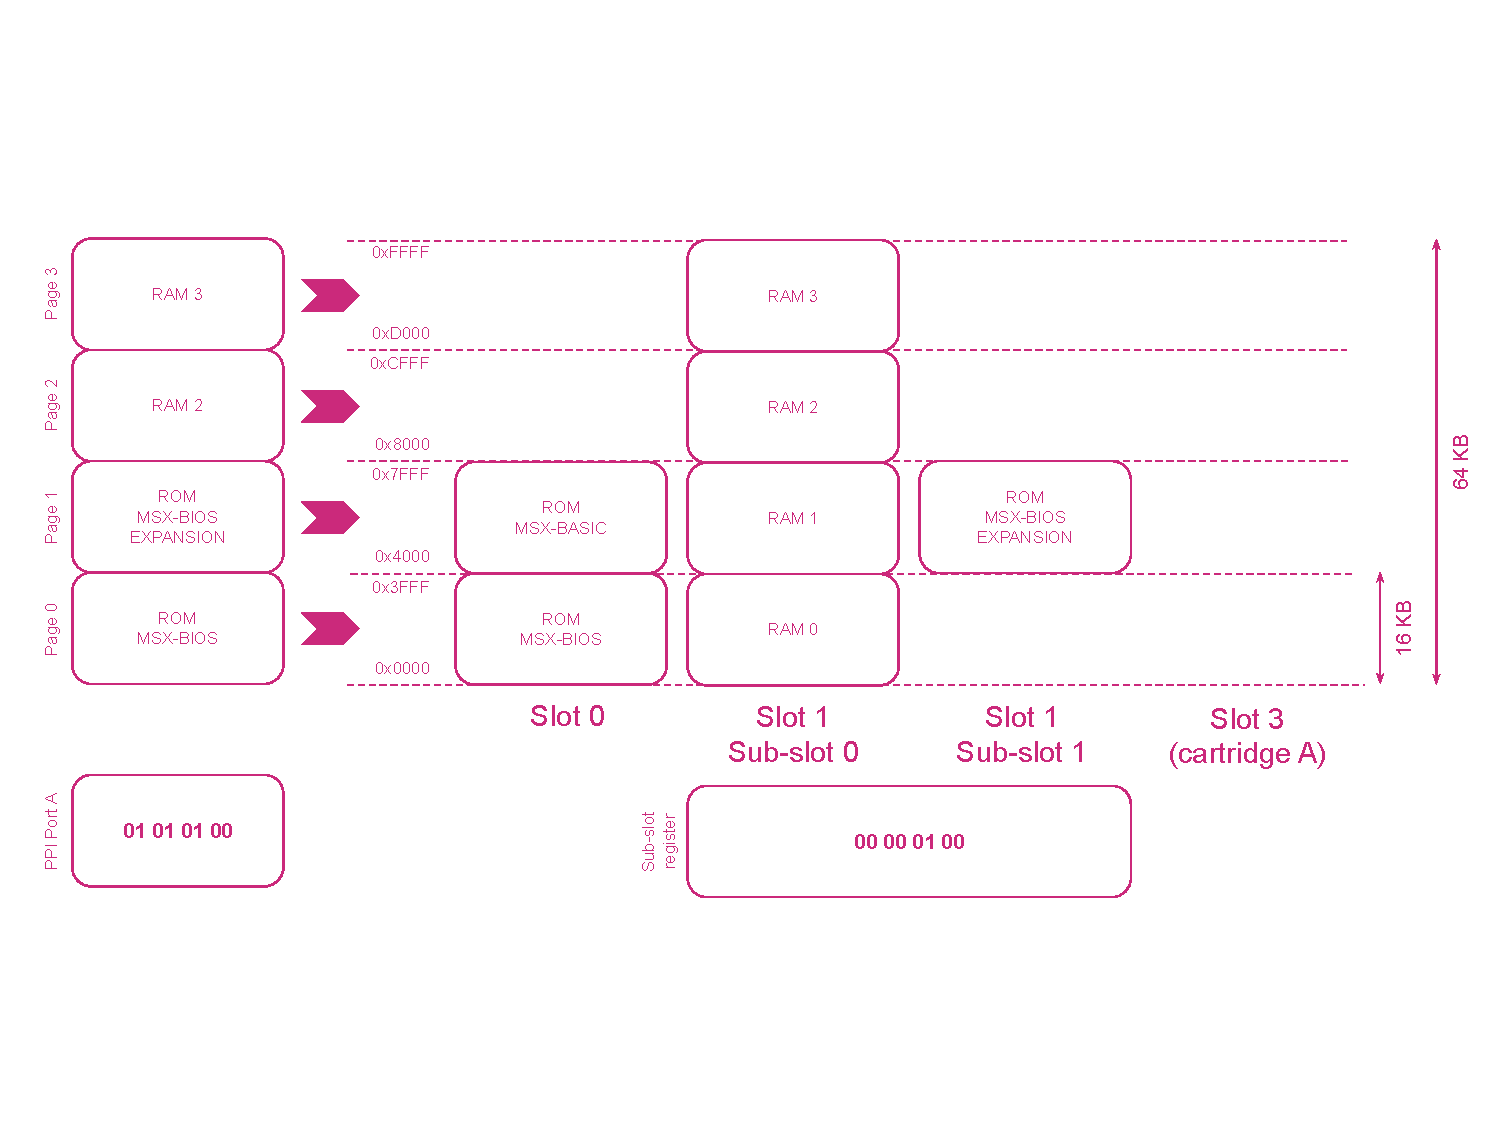
\includegraphics[width=1\linewidth,trim={0cm 100 0 80}]{images/figures/msx-mem-slotssec}
	\caption{MSX secondary memory slots configuration}
	\label{fig:msx-mem-slotssec}
\end{figure}

If we want to map the page 2 and 3 to RAM, we must:
\begin{itemize}
	\item Configure the pages 2 and 3 to use the primary slot 1. This means writing the value 0b0101xxxx to the PPI port A.
	\item Configure the register of primary slot 1 to use sub-slot 0 for pages 2 and 3. This means writing the value 0b0000xxxx to the register of slot 1 at address 0xFFFF.
\end{itemize}

Analogously, to have the MSX-BIOS Expansion accessible at page 1, we must:

\begin{itemize}
	\item Configure the page 1 to use the primary slot 1. This means writing the value 0bxxxx01xx to the PPI port A.
	\item Configure the register of primary slot 1 to use sub-slot 1 for page 1. This means writing the value 0bxxxx01xx to the register of slot 1 at address 0xFFFF.
\end{itemize}

As you might figure out, accessing the address 0xFFFF in certain primary slots is tricky. A primary slot will respond to that address only when page 3 is configured to use that slot because address 0xFFFF belongs to page 3. Thus, in certain configurations it is necessary to configure the page 3 to use that slot first, and then write to the address 0xFFFF to set the sub-slot configuration. After this, we must restore the previous configuration of the primary slots to leave the things in a consistent state. \\

But the problems do not end there. As we mentioned above, the MSX standard does not impose any specific slot layout. The users and their software must not make any assumption about where RAM or ROM is located. This implies the software, including the MSX BIOS, must be able to discover where the memory is. This can be done with a subprogram that scans the slots looking for RAM memory. But how can it determine if a primary slot is expanded or not? Consider an expanded slot has a register at address 0xFFFF. But a primary slot may have a RAM memory in this very address. In both cases, this address can be written and read. How could the software say if this is a cell in a RAM memory chip or it is a hardware register?\\

The MSX standard has an answer to this. It states that the hardware register of an expanded slot must respond by inverting the contents when the register is read by the CPU. Thus, if the software writes 0b01010101 to the address 0xFFFF of a primary slot and immediately after that it reads back what was written, there are three possible results:

\begin{itemize}
	\item 0b01010101. The same value that was written. It means this slot contains RAM and it is not expanded.
	\item 0b10101010. The value that was written with its bits inverted. It means this slot is expanded.
	\item Any other value. The slot does not have anything responding to write operations at 0xFFFF. It means indeed the slot is not expanded. It might be a primary slot with ROM at page 3, the slot is not connected, or it is a cartridge slot that has nothing plugged.
\end{itemize}

As you can see, the memory slots system is rather complex but powerful. Each memory page can be mapped to a maximum of 16 different slots. This is a total address space of 1 megabyte of memory. Not bad considering that 640 KB ought to be enough for everybody. 

